% !TeX root = ../thuthesis-example.tex

\chapter{Open-Source LAMP hardware}
The previous chapter have described the design and manufacture of freeze-dried QUASR-LAMP reactions allowing the diagnose of SARS-CoV-2 in LMICs. However, as we introduced in the chapter's conclusions, there is still the need for equipment to incubate and analyze the reactions. While incubation requires relatively inexpensive equipment (e.g., a pot and sous vide cooker), the development of the reactions still requires a transilluminator.

Despite previous work by the group to create low-cost transilluminators for GMO detection based in QUASR-LAMP\cite{guy_aidelberg_gmo_2018}, our aim during this thesis was to integrate both the incubation and development equipment into a single unit. For manufacturing the system, we used digital fabrication tools currently spread along the LMIC's maker labs such as Kumasi Hive (Ghana) or the Ongola fab lab (Cameroon).

The second part of this chapter describes the creation of low-cost equipment to carry out Real-Time LAMP experiments, in which the fluorescence generated by the reactions is measured analogically as the incubation progresses. This equipment allows moving forward from qualitative LAMP tests to quantitative measurements (qLAMP), expanding the horizon of possibilities for the assays that can be carried out in remote developing regions.

Both systems are documented in the GitLab of the Open Bioeconomy Lab\cite{francisco_javier_quero_lombardero_open_2021}, an interdisciplinary research group based in the Department of Chemical Engineering and Biotechnology at the University of Cambridge, but also working closely with researchers in Tsinghua University, Cameroon and Ghana. This whole project has been carried out and co-funded as part of OBL, and through its members working on the ground, we have received invaluable feedback and advice.
\newpage

\section{WaterBath}

The idea behind the WaterBath is to serve as a portable and affordable solution to incubate and visualize LAMP amplifications. As it is ideated to work on remote developing regions, the total production price is approximately 5€.

Water is used as the incubating medium because its excellent properties as a thermal conductivity material that makes it a standard in the biotech industry. First, liquid incubation offers higher thermal conductivity than air incubation. Second, from all the materials that keep the liquid state at room temperature, water offers unusually high specific heat capacity, allowing efficient heat transfer over distance with low rates of mass transfer\cite{company_nalco_1979}.

 \begin{figure}[b]
    \centering
    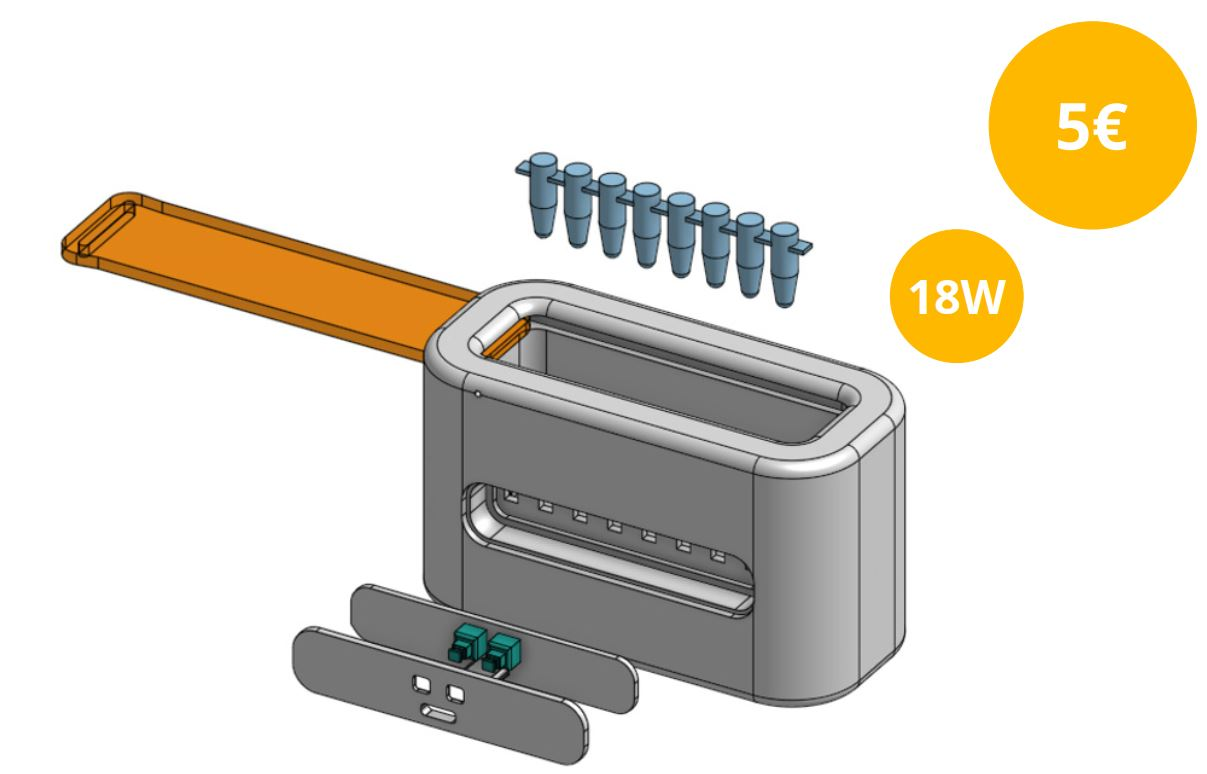
\includegraphics[width=0.95\textwidth]{figures/WaterBath.JPG}
    \caption{Exploded view of the water bath. The system's final price is around 5€ and consumes just 18W, making it possible to power it with an external battery.}
    \label{Exploded view water bath}
\end{figure}

The designed equipment serves as a water bath for incubating the reactions at constant 63ºC, that can be changed by tuning an internal resistor. Following the incubation, the results can be easily analized with an integrated transilluminator made out of 470nm LEDs that light the central chamber from the side, together with a top orange filter that only let go through the green fluorescence of the reactions, filtering out the light from the LEDs. For maintaining the simplicity and the low price of the system, all the electronics are analogic, except the USB-C power deliver negotiator, which allows the system to be supplied by a type C charger able to deliver 9V/12V or even a power bank.

All the designs and manufacturing files can be obtained from the projects' GitLab\cite{francisco_javier_quero_lombardero_open_2021}.


\subsection{Working principle}
The operating mechanism of the water bath is relatively simple; after preparing the QUASR-LAMP reactions, the water bath is filled, closed with the acrylic filter and the incubation button is pressed. A light will turn on while the water bath is heating up. Once the light turn off, the reactions are placed in the eight tube-strips little holders, leaving them incubating for one hour.

Once incubated, the hot water is emptied, and the container is filled with cold water. After waiting 5 minutes for the reactions to cool down (QUASR-LAMP needs to be read cold \cite{ball_quenching_2016}), the second button is pressed, lighting up the side LEDs. This action will illuminate the inner chamber, and the resulting fluorescence will be visible from the top of the water bath if the reactions are positive (Figure 4.2).

 \begin{figure}[b]
    \centering
    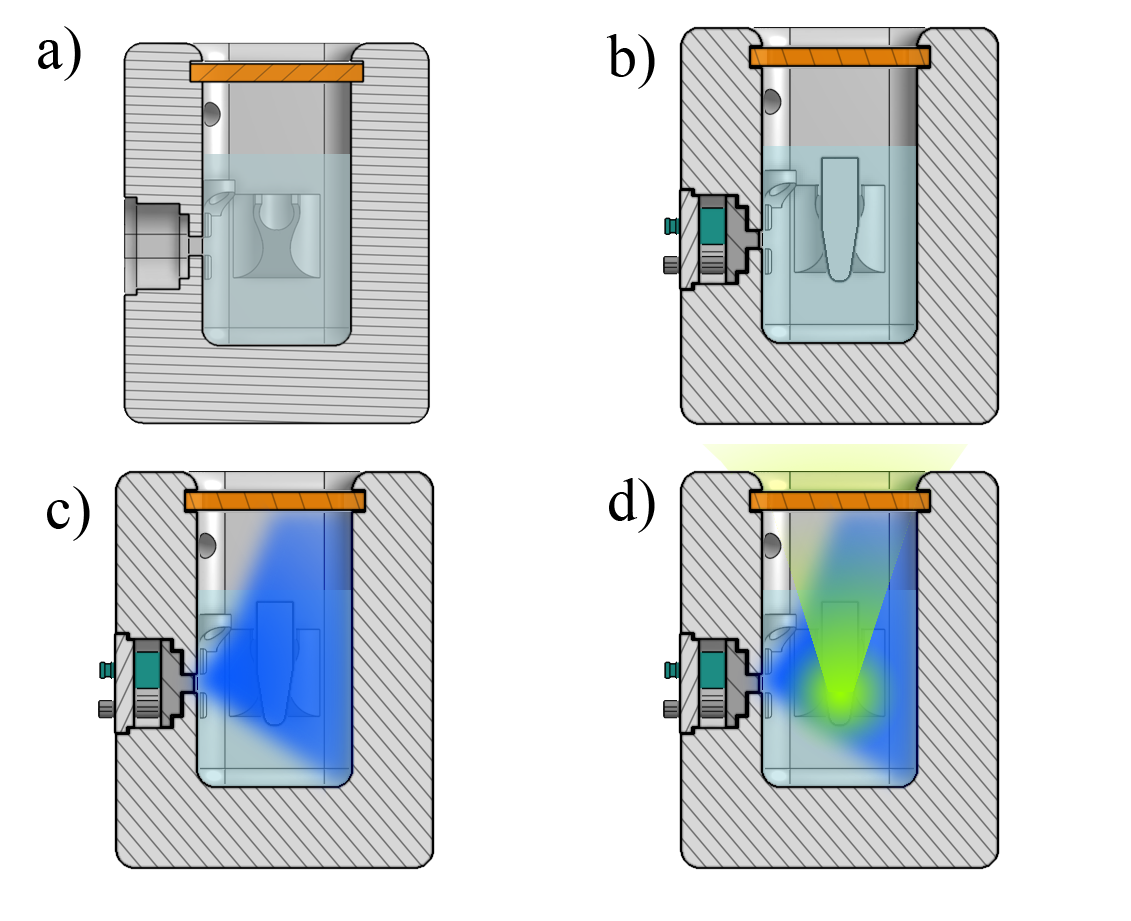
\includegraphics[width=1\textwidth]{figures/WorkingPrinciple.png}
    \caption{Working principle of the water bath. a) The water bath is filled with water, closed and is preheated. b) The reactions are introduced in the holders, and the water bath is closed. c) After one hour, the results are visualized thanks to the activation of the lateral LEDs d) If the reaction is positive, the fluorescence can be observed from the top.}
    \label{Working Principle Water Bath}
\end{figure}

\subsection{Parts}
\subsubsection{Electronics}
The electronics are based on a standard analogue temperature control system, which is robust and straightforward, does not need to be programmed and is exceptionally cheap. It relies on the control of a heater element through a MOSFET regulated by the NE555 chip (Figure 4.3(A)).

The system has been designed for soldering most of the components using the manufacturer's SMT service and parts catalogue (JLCPCB, People's Republic of China), except the USB type C port driver (IP2721\_MAX12), which is readily available from various distributors.

As typically the suppliers only accepts SMT soldering on one side of the PCB, the system has been designed in two parts, which must be separated and soldered back to back. One side consists of the LEDs that illuminate the internal water bath camera, and the other side consists of the rest of the system, the USB connector and the user interface buttons, that faces the exterior of the machine.

The system works with the Type C standard (Figure 4.3 (B)), supporting a 9/12V power supply and allowing the water bath to be plugged on with phone chargers or a power bank capable of supplying these voltages. All schematics and fabrication files can be found on the Open Source Hardware Lab platform\cite{francisco_javier_quero_lombardero_lamp_2021}.

 \begin{figure}[b]
    \centering
    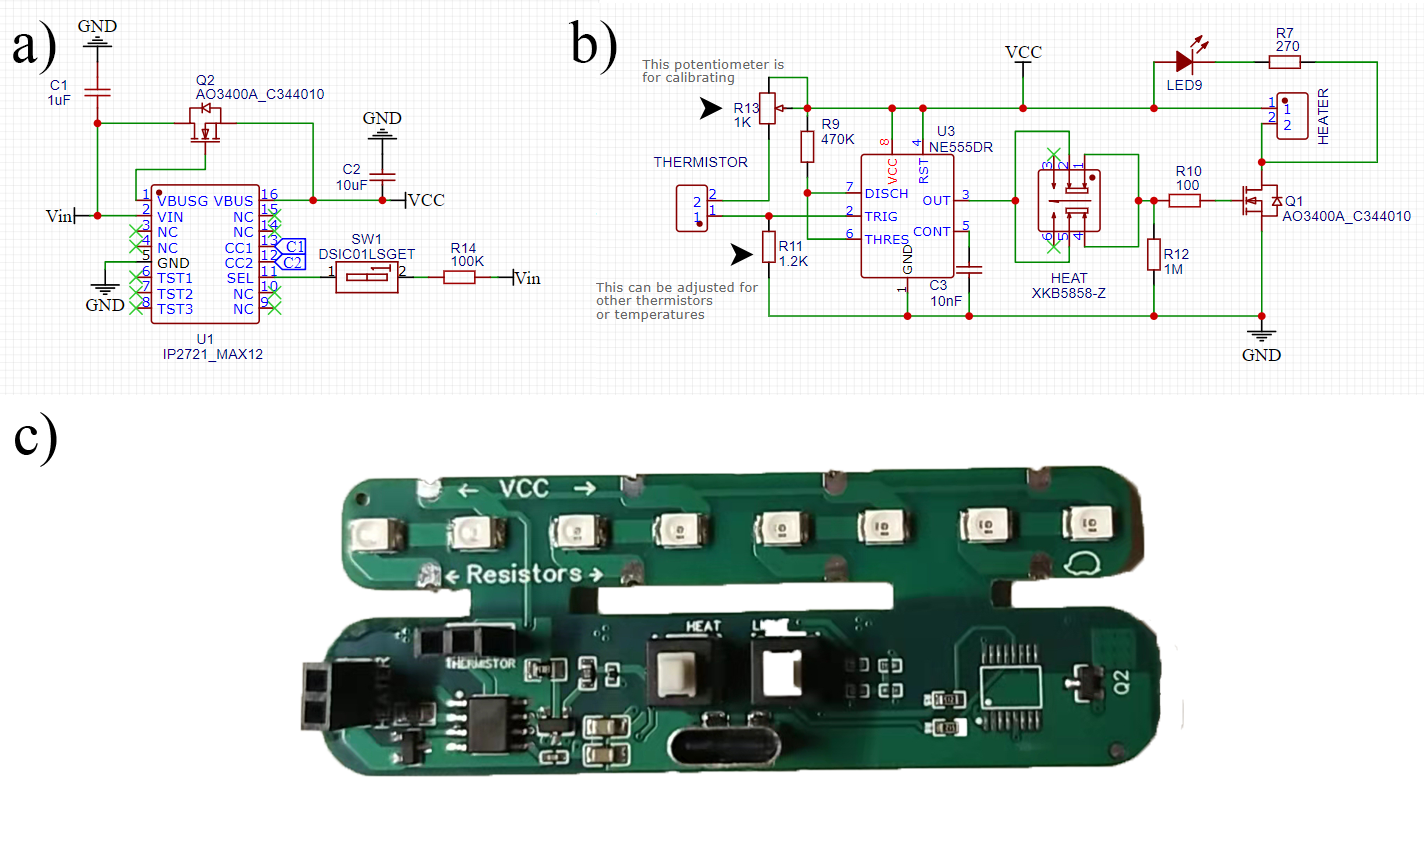
\includegraphics[width=0.9\textwidth]{figures/electronica.png}
    \caption{Schematics of the a) USB C regulator circuit and b) temperature control circuit. c) Printed Circuit Board as it comes from the manufacturer (Without the IP2721 chip). Additional information can be found on the project GitLab\cite{francisco_javier_quero_lombardero_open_2021}.}
    \label{Schematics Water Bath}
\end{figure}

\subsubsection{Case}
The biggest challenge in designing the structure of the water bath lay in the search for affordable materials that stay robust at the temperature at which they needs to work. The primary and most widespread 3D printing technique is Fused Deposition Modeling (FDM) based on melting a plastic filament and then depositing it, with a three-axis motorised system, layer by layer until the final object is created. The major problem with this technique is beside the nature of the materials used. Because they are designed to melt at around 200ºC, they have a glass transition (the temperature at which they begin to deform) of less than half that temperature. Therefore, because 63°C needs to be maintained during the LAMP reaction, most of the traditional FDM materials suffer from deformation, making their use unfeasible.

\begin{figure}[b]
    \centering
    \includegraphics[width=0.65\textwidth]{figures/sla.png}
    \caption{Resulting case from an SLA printing. Model can be found at OnShape platform for SLA\cite{francisco_javier_quero_lombardero_sla_2021} and FDM printing \cite{francisco_javier_quero_lombardero_fdm_2021}.}
    \label{3D printing}
\end{figure}

One possible solution is to employ other printing methods that use non-melting based materials. One such technique is stereolithography 3D printing (SLA). This technique uses resins that polymerise due to exposure to light, typically consisting on blue or shorter wavelengths. SLA printing equipment uses a laser beam to polymerise the final part layer by layer inside a tank. We experimented with creating the case employing a Formlabs SLA printer (and their compatible resin) with a satisfactory result (Figure 4.4). Unfortunately, although we modified the 3D model to be hollow and use less material\cite{francisco_javier_quero_lombardero_sla_2021}, the price of the Formlabs resin is still too elevated for this application, resulting in a part costing more than 10€.


Although a possible solution is to go to lower-cost SLA printing brands (e.g. Creality or Anycubic), another restricting factor relies on the fact that this 3D printing technology is less widespread in maker labs, especially in developing countries. For this reason, we experimented with FDM printing materials that have a glass-transition temperature above 80ºC. One such material is PETG, which in practice gave us good results. Furthermore, the prices of printing the case with PETG are less than a \$1. Models for FDM 3D printing can be found on the OnShape platform\cite{francisco_javier_quero_lombardero_fdm_2021}.

\subsubsection{Heater design}
Aiming to find a solution that adapts to our needs in terms of power consumption, shape and price, a custom made PCB heater was designed. The heater shape was derived from the bottom of the waterbath and the trace width and length was calculated using the following formula:


\begin{equation*}
\centering
R = \rho \cdot \frac{L}{T \cdot W} \cdot [1 + \alpha (temp -25)]
\end{equation*}
\vspace{12pt}
\begin{center}
    \small{\textbf{Where:} $R$ = resistance, $ρ$ = resistivity, $L$ = length, $T$ = trace height, $W$ = trace width, \\$α$ = temperature coefficient, $temp$ = temperature}
\end{center}
\vspace{12pt}

We calculate the trace to consume around 1.5 A at 12V and 60ºC. The resulting resistance is 8Ohm with a length of 217cm and a width of 0.16mm. The PCB was manufactured using aluminium as the support (JLCPCB, People's Republic of China). In the heat uniformity analysis the PCB heater performed well, with less than one degree of difference between the perimeter and the center (Figure 4.5). All schematics and fabrication files for the heater can be found on the Open Source Hardware Lab platform\cite{francisco_javier_quero_lombardero_lamp_2021}.

\begin{figure}[b]
    \centering
    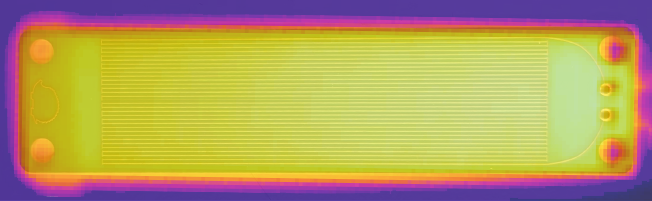
\includegraphics[width=0.7\textwidth]{figures/heat uniform.png}
    \caption{Heat uniformity analysis of the designed heater.}
    \label{Heat uniformity}
\end{figure}
\newpage

\subsubsection{Optics}
The optics of the water bath are based in three main components (Figure 4.6):
\begin{itemize}
\item The light source, consisting of a 470nm LED (Mouser Electronics, UK).
\item The QUASR-LAMP probes containing fluorescein, a fluorophore that absorbs at the blue wavelength of the source and emits in a green one.
\item The filter at the top of the water bath, which allows only the green light to pass through, separating the fluorophore's emission from the light source. 
\end{itemize}
\vspace{12pt}
\begin{figure}[h]
    \centering
    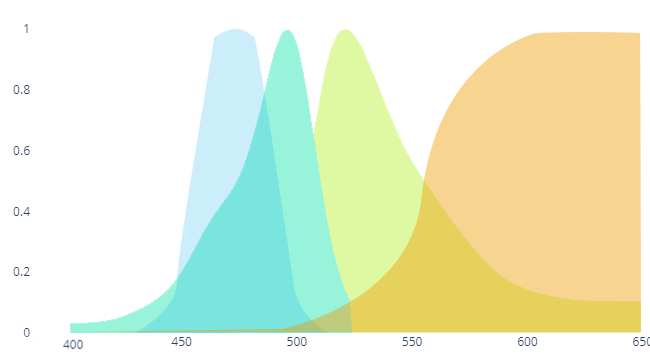
\includegraphics[width=0.8\textwidth]{figures/wavelengths.png}
    \caption{Spectrum from the different components of the optic system. \textcolor{blue}{Blue}, LED emission; \textcolor{Turquoise}{Turquoise}, Fluorescein absorbance; \textcolor{GreenYellow}{Green}, fluorescein emission; \textcolor{Orange}{Orange}, spectrum allowed by filter.}
    \label{wavelengths}
\end{figure}
\vspace{12pt}

Different solutions were explored to solve the challenge of finding an affordable filter with good performance. Firstly, filters from a manufacturer of theatrical lighting products (LeeFilters, UK) were explored. The manufacturer was chosen because of their vast range of filters, the excellent price (at a few euros per $m^2$) and outstanding characterisation of their absorption spectrum. The filters were mounted on a 3D printed holder that fitted into the top slot of the WaterBath (Figure 4.7(A)). The main issue we faced with this system is their tedious fabrication and the fragility of the result. For this reason, we found a better solution cutting the entire filter out of a piece of 3mm thick transparent orange acrylic (Figure 4.7 (B)).

\begin{figure}[h]
    \centering
    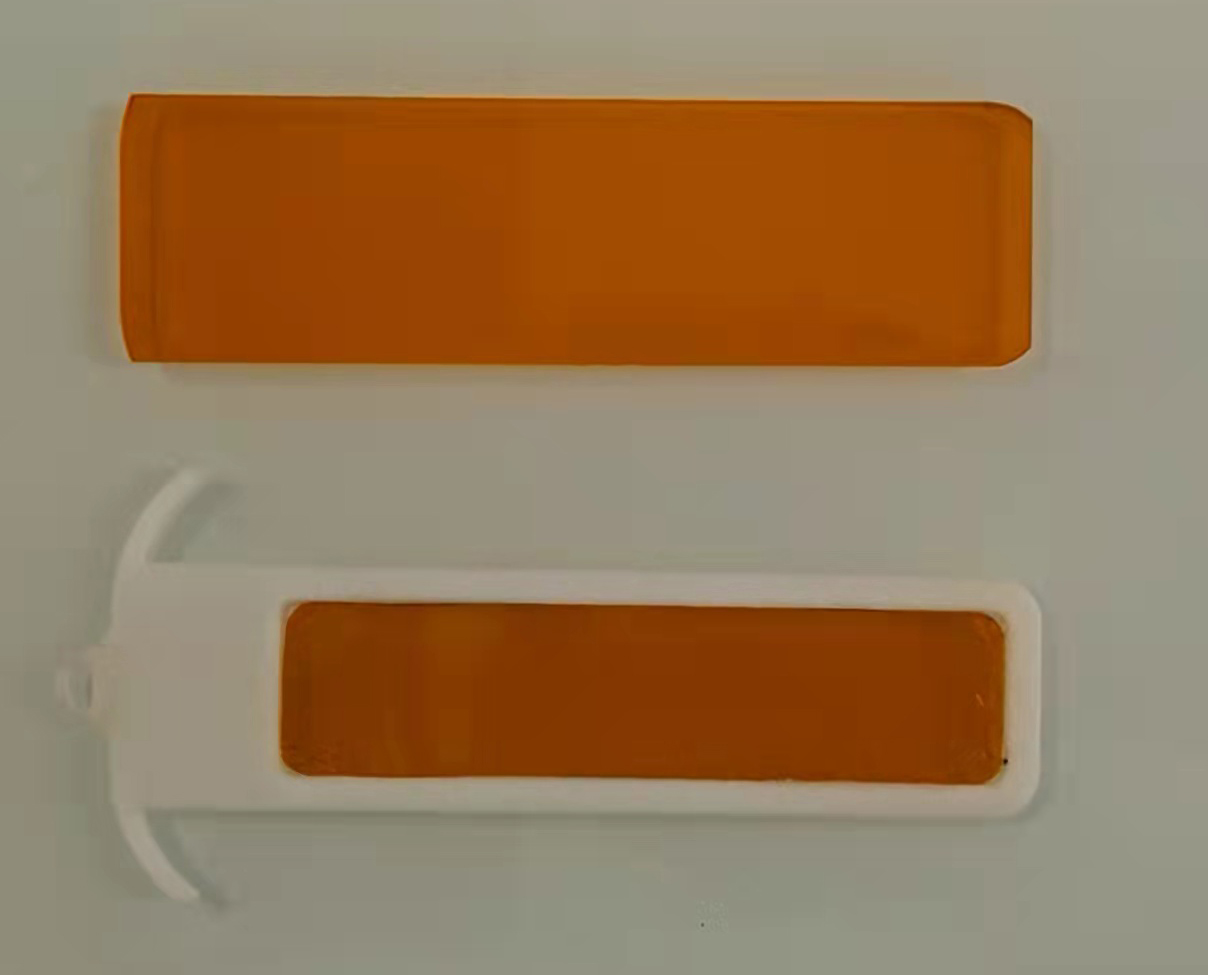
\includegraphics[width=0.8\textwidth]{figures/filters.jpg}
    \caption{The two solutions used as a filter for the waterbath. At the top is a filter cut entirely from transparent orange acrylic. At the bottom is a low-cost filter for theatrical lighting (LeeFilters, UK) on a 3D printed support.}
    \label{filter}
\end{figure}

\newpage
\subsection{Results and conclusions}
The water bath was benchmarked against the combination of a thermocycler (BioRad, US) and a low-cost transilluminator (IORodeo, US), comparing their performances to incubate and analyze QUASR-LAMP reactions (Figure 4.8). Combined with Corona Detective reactions, both systems showed a detection limit of one viral copy per uL. These results demonstrate the ability of the kit to detect coronaviruses at a meagre cost, with a water bath of \$5 and reactions of less than \$2. Furthermore, the system is portable and can be supplied by a power bank battery. However, more results are needed to characterize the number of reactions per charge. 

As a final point, the hardware has been conceived and designed to be replicated in locally by the use of inexpensive digital manufacturing techniques. We are working with the maker labs near our collaborators in LMICs to try to replicate the system on the field and collect feedback on usability for future versions.

\newpage
\null
\vfill
\begin{figure}[h]
    \centering
    \includegraphics[width=0.95\textwidth,keepaspectratio]{figures/waterbath results.png}
    \caption{(Top-left) Results of Corona Detective amplification testing the water bath. (top-right) Comparison of the amplification results between the water bath and a commercial thermocycler employing an external transilluminator. Both results show equivalent, with a detection limit of 20 copies per reaction (~1 viral copy per microlitre). (Bottom) Image depicting the reaction preparation process prior to incubation.}
    \label{wb results}
\end{figure}
\vfill


\newpage

\section{Real time LAMP equipment}
As mentioned in the first chapter, Real-Time PCR is the current gold standard in the diagnosis field. Reading the fluorescent signal constantly at each amplification cycle is the essential characteristic of this technique, allowing the kinetics of the reaction to be observed in detail. The advantages of this technique compared to end-point reactions are numerous. First of all, the real-time measurement allows catching false positives that may have been generated in the last moments of the reaction due to aberrant amplification (Figure 4.9). Secondly, it makes possible the optimisation of the different features of a reaction (different primer sets and their ratios or enzyme and magnesium concentrations, among others) since it offers the opportunity to compare precisely the different performances associated with the combinations of the features.

\begin{figure}[b]
    \centering
    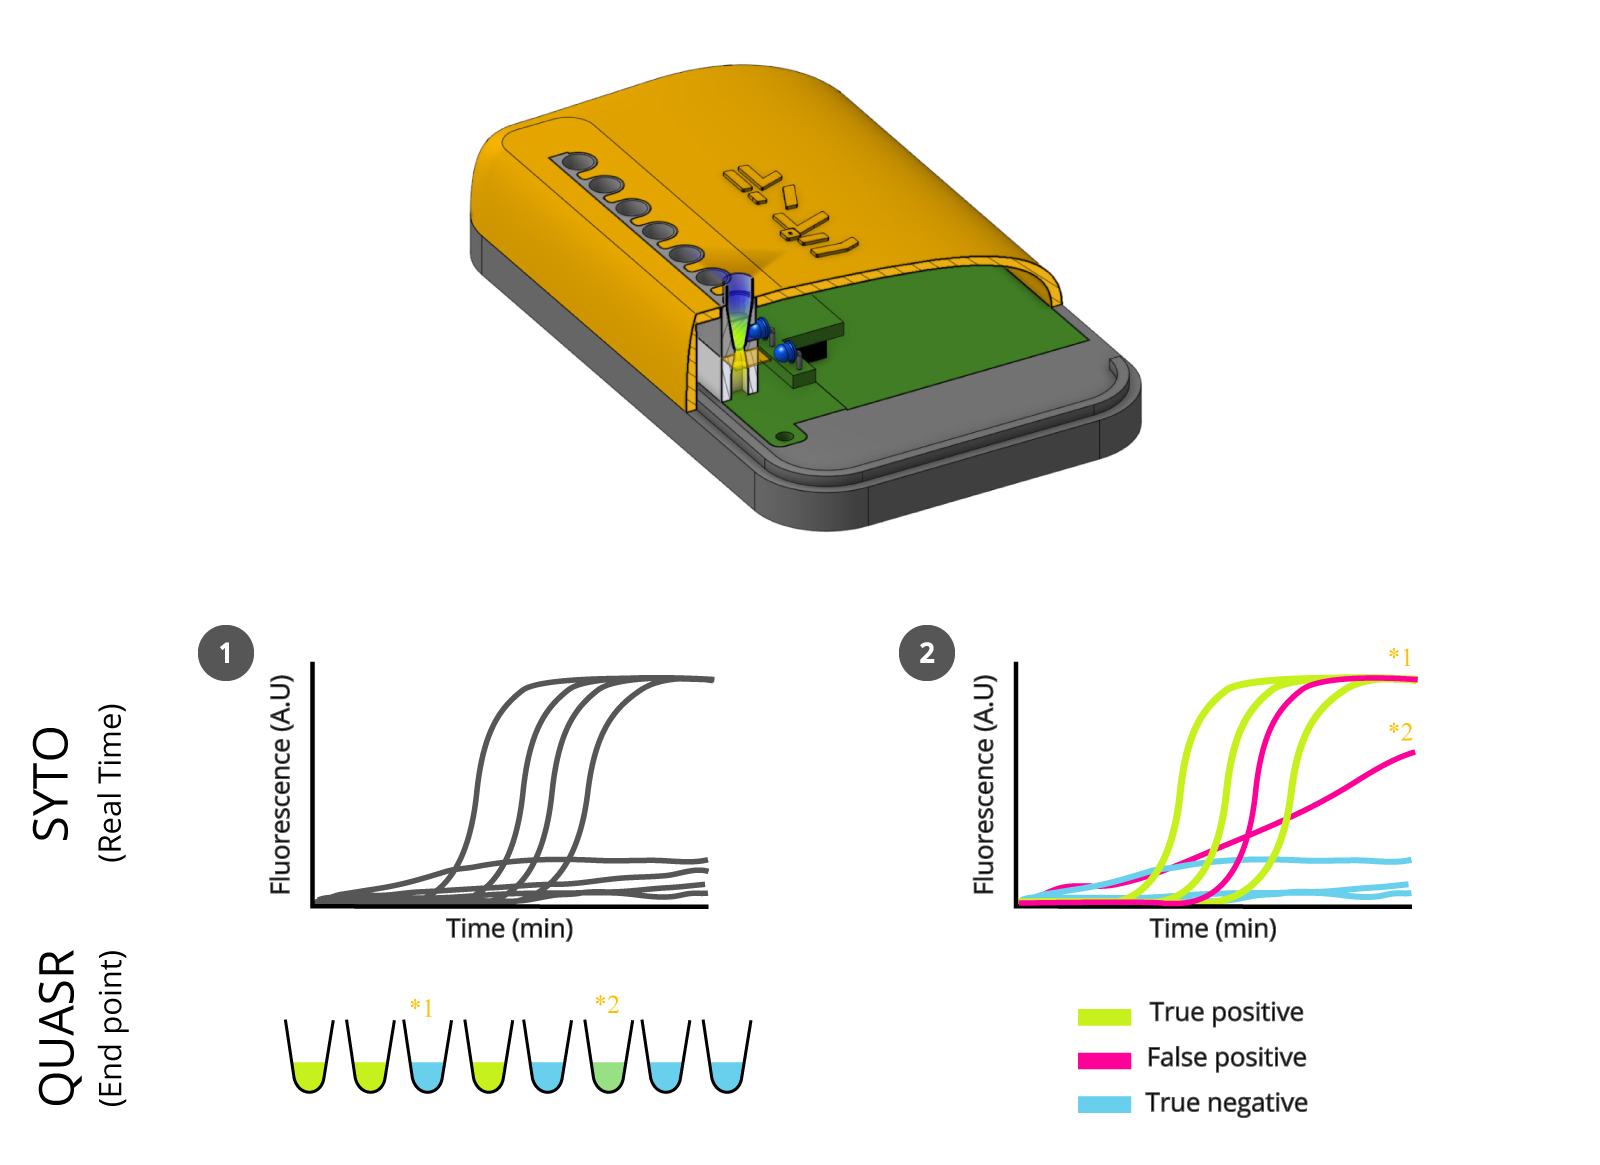
\includegraphics[width=0.95\textwidth,keepaspectratio]{figures/qlamp.png}
    \caption{(Top) Section of the Real-Time LAMP machine. (Bottom) Detailed process of false-positive filtering using real-time QUASR amplification. (1) Reactions are amplified, measuring SYTO9/82 fluorescence in real-time and cooling down the reactions to obtain an end-point value of the QUASR fluorescence. (2) The unspecific amplifications, spotted thanks to the end-point result of the QUASR detection and the real time measurements, are filtered from the real-time amplification data.}
    \label{qLAMP}
\end{figure}

The fundamental problem of Real Time PCR technique is the expense of the equipment. If a normal thermocycler costs around \$3000, a qPCR machine costs in the order of magnitude of \$30.000, which is prohibitively expensive in areas where even a stable electricity supply is not assured. During this thesis, the last goal to address has been to develop a machine that allows real-time quantification of isothermal amplification in real-time, affordably and straightforwardly, to ultimately enable remote low resource areas to perform quantitative nucleic acid testing. 

The development of this equipment is still in progress, so the results of this thesis are preliminary, and the scientific publication in which they will be included is in preparation. 


\subsection{Design}

The equipment is divided into six subsystems (Figure 4.10):

\begin{itemize}
\item \textbf{The microcontroller module}, consisting of an ESP32 that allows control of the machine through the local network, acting as a server and allowing the end-user to interact with the system through a simple web page. 
\item \textbf{The lighting module}, consisting of 8 blue LEDs emitting at 470nm and governed by a standard LED driver in the maker ecosystem (WS2814, WorldSemi).
\item \textbf{The fluorescence readout module}, consisting of a photodiode, a transimpedance amplifier circuit and a dedicated 16-bit analogue-to-digital converter. Prior to signal measurement, the light is filtered with a LeeFilter number 105. 
\item \textbf{The incubation module}, governed by a Proportional-Integral-Derivative (PID) algorithm that activates a Kapton-based heating element. The heating element is sticked to a 3D printed aluminium piece (Jiinsoon LTC, People's Republic of China) that holds the 8-tube strips with the reactions and channels the resulting fluorescence to the light-sensing module.
\item \textbf{The power supply module}, similar to the one previusly described in the water bath section. It is based on the USB type C standard and allows the user to power the entire device with a phone charger or even a power bank.
\item \textbf{The housing case}, 3D printed on PETG using an FDM printer (Prusa i3, Prusa Research).
\end{itemize}

All the detailed schematics, manufacturing files and 3D models can be found in the GitLab page of the project \cite{francisco_javier_quero_lombardero_open_2021}.

\newpage
\null
\vfill
\begin{figure}[h]
    \centering
    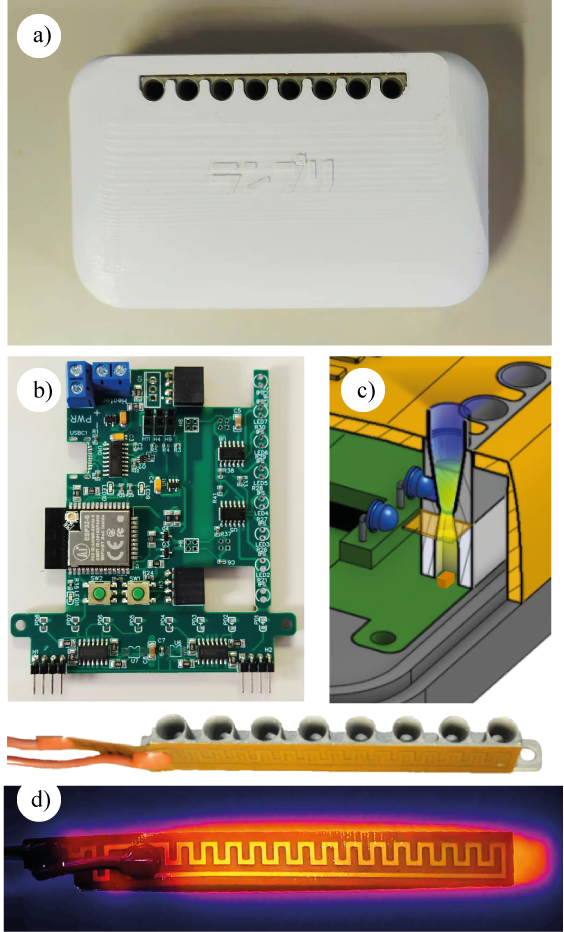
\includegraphics[width=0.55\textwidth,keepaspectratio]{figures/qLAMP-parts.png}
    \caption{Detail of the Real-Time LAMP machine modules. (a) Case of the machine 3D printed in PETG. (b) Detail of the electronics. The PCBs from the different modules come together, so they need to be broken apart and joined using the connectors. The ESP32 microcontroller governs all the modules and connects the machine to the local network, allowing the user to control the machine and see the results in real-time through a phone or a computer connected to the same local network. (c) Detail of the optics module. The LEDs light the reaction tubes from the side. If the reaction is positive, and therefore fluorescence is generated, the light goes down through a hole in the metal piece, crosses the high pass filter, and reach the photodiodes in the sensor PCB below the holder. (d) Detail of the metal holder with the Kapton heater stuck in the back (Top). Heating uniformity analysis of the Kapton heater (Bottom). All the electronic schematics and 3D models can be obtained from the Gitlab repository of the project\cite{francisco_javier_quero_lombardero_open_2021}.}
    \label{qLamp parts}
\end{figure}
\vfill


\newpage

\newpage
\subsection{Results and conclusions}
As previously introduced, this equipment is still under development, and therefore the results are preliminary. Therefore, they should be understood as a first sample of the system's future potential and not as a final result. 

A simple assay was performed using SYTO9 as the signal generator to test the system's ability to measure the amplification in real-time (Figure 4.11). Despite preliminary results showing a sensitivity with a vast margin for improvement, the system successfully measured the signal in real-time in this first test. This data indicates that the prototype is on track to become a real-time LAMP machine successfully. However, this results evidenciate the need for further work after this thesis, to reduce noise, increase sensitivity, and benchmark the system against the RT-PCR gold standard.   

\begin{figure}[b]
    \centering
    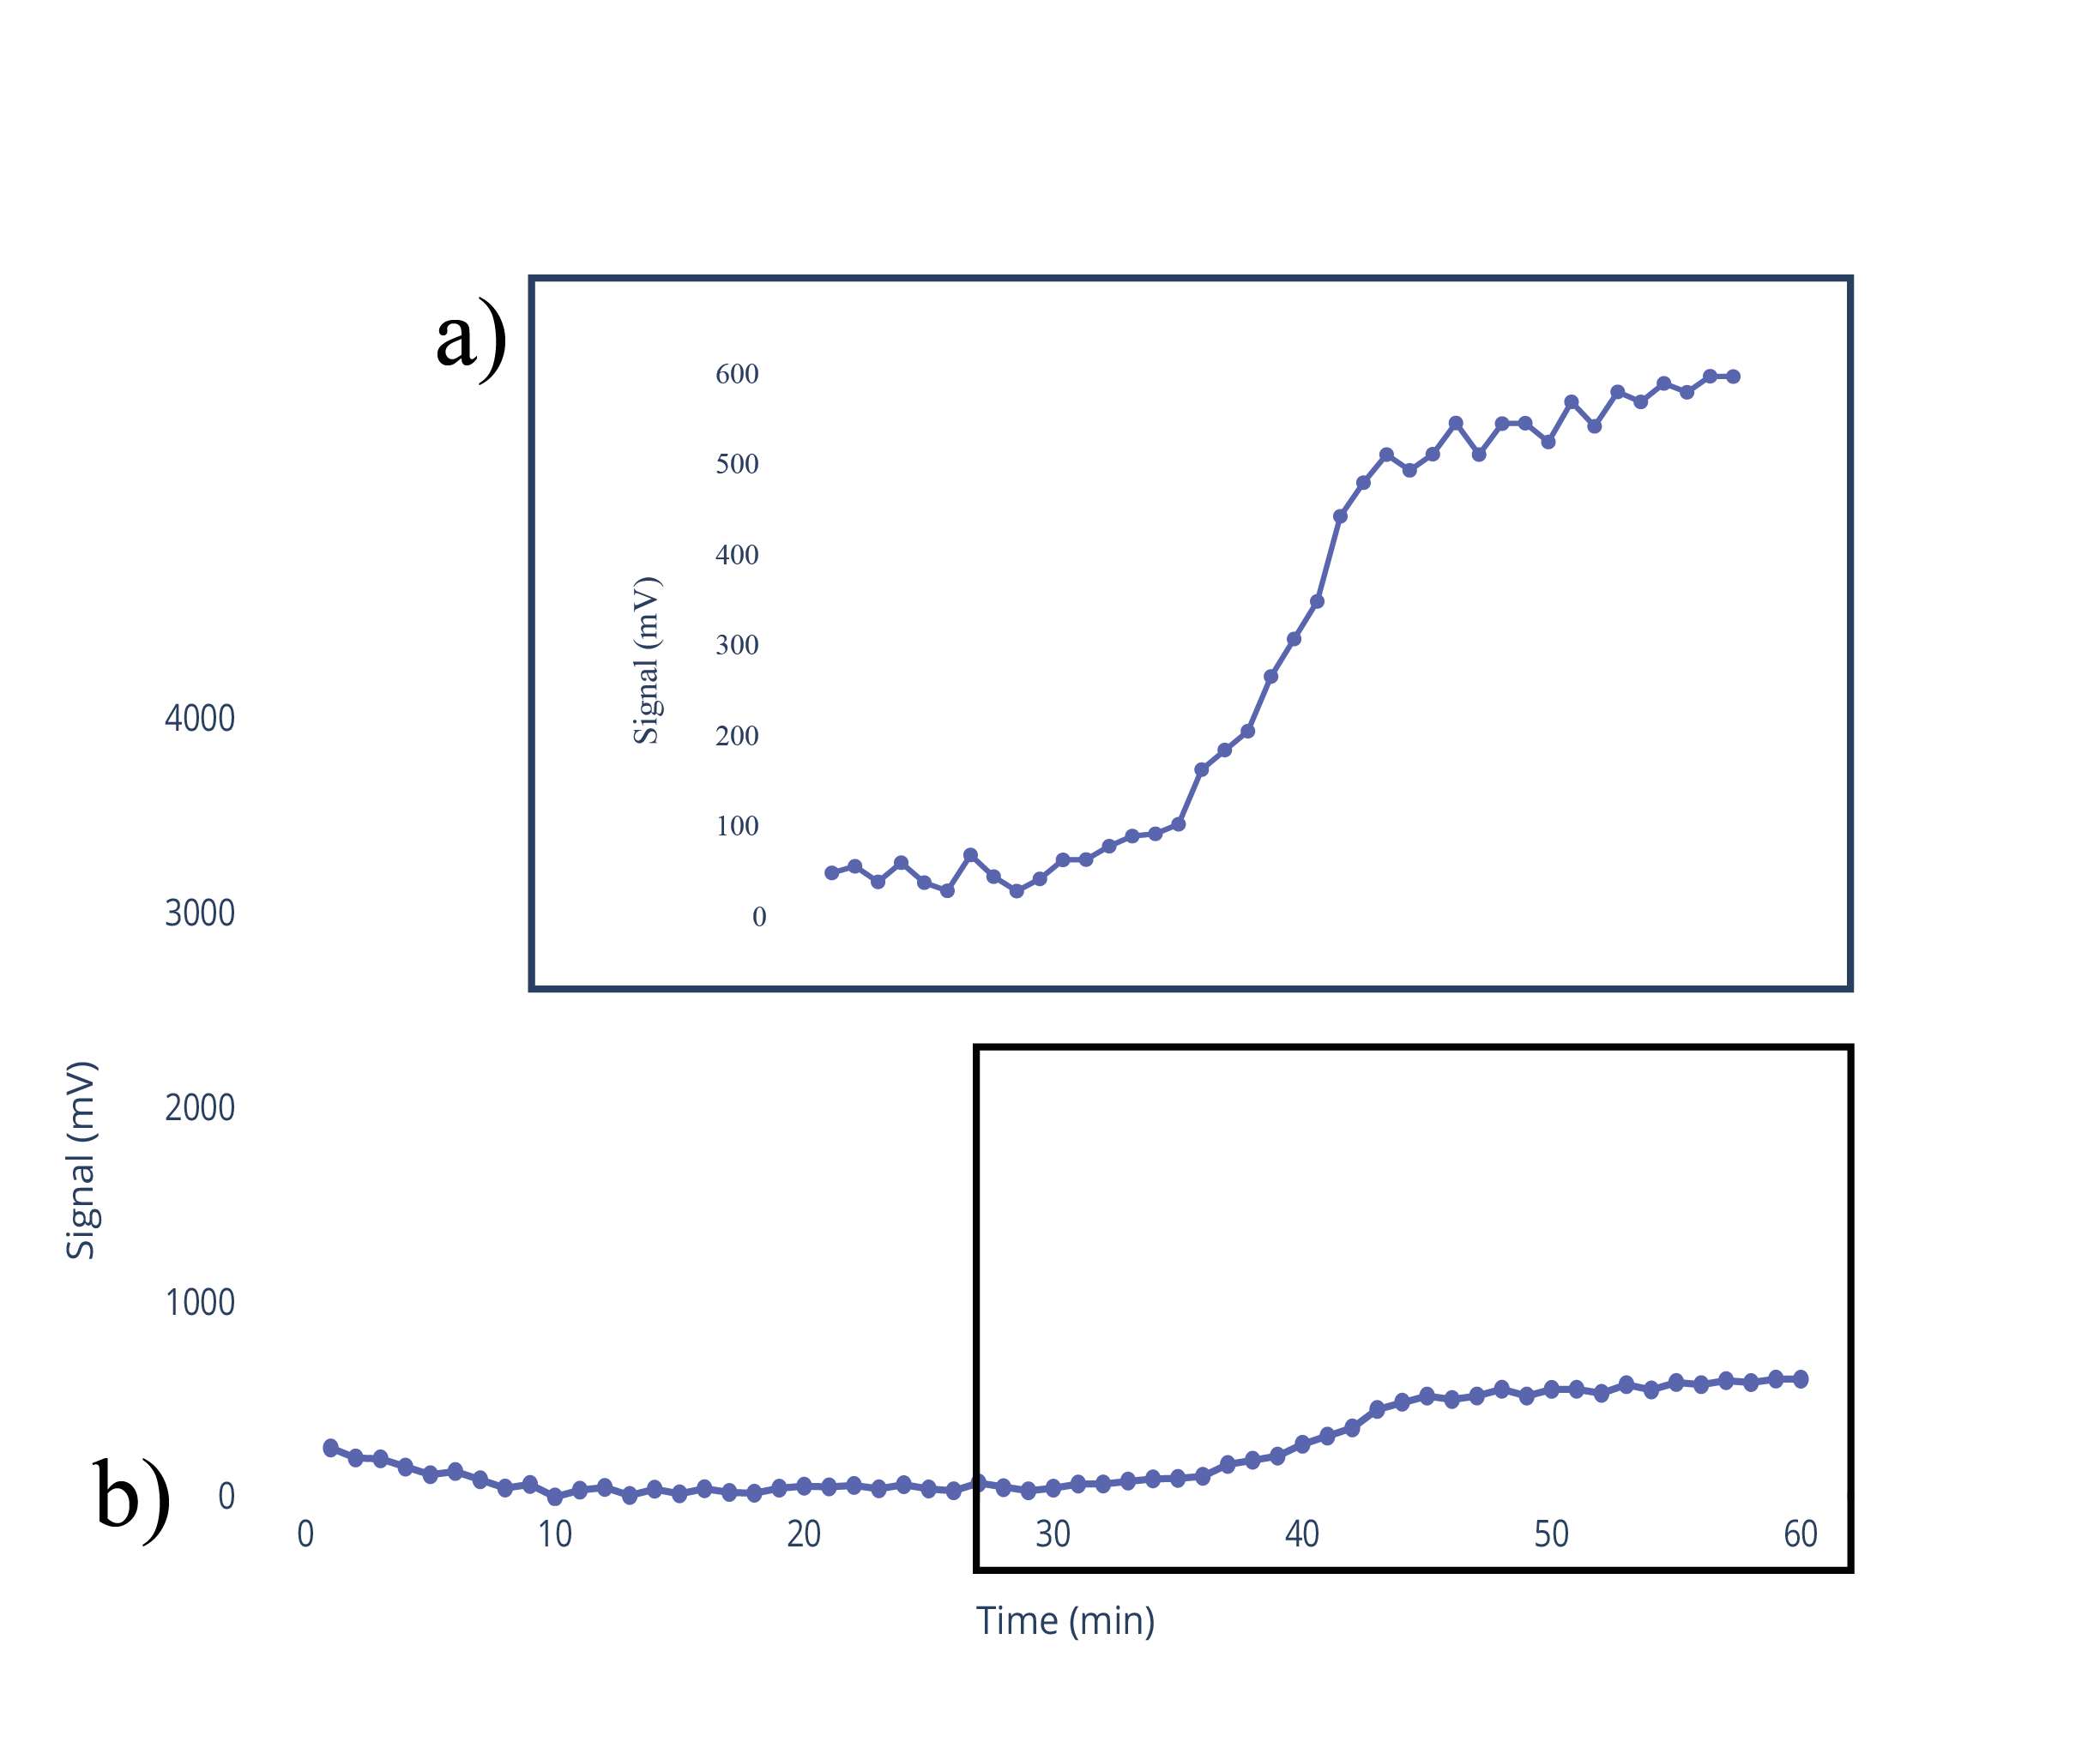
\includegraphics[width=0.9\textwidth]{figures/signal.png}
    \caption{Although the signal can be distinguished in a real time amplification-like result (a) the signal is still small compared with the entire range of the system (b). This results evidenced the need of continuing experimenting with solutions that helps increasing the signal.}
    \label{qLAMP signal}
\end{figure}

The total price of manufacturing the system on a small scale (using digital manufacturing techniques) is broken down in Table 4.1. It should be noted that the price of the system is about 3 orders of magnitude lower than a commercial Real Time PCR machine.

\begin{table}[]
\centering
\begin{tabular}{rl}
\textbf{Component}    & \textbf{Price (USD)} \\
Assembled electronics & 45                   \\
3D printed alluminium tube holder           & 7                    \\
3D printed printed case      & 1                    \\
Kapton heater         & 1                    \\
Optic filter          & \textless{}1         \\
\textbf{Total}        & \textbf{54}         
\end{tabular}
\caption{Breakdown of manufacturing prices.}
\end{table}


It is also important to mention that, for performing real-time measurements, the QUASR-LAMP technology presents a critical problem; the fluorescence needs to be read in cold or, at least, at room temperature. As mentioned in the first chapter, in QUASR-LAMP the quencher-fluorophore combo is designed with a melting temperature significantly lower than the incubation temperature, aiming that the quencher probe does not compete for the primer during the reaction. Because of that, measuring the fluorescence at room temperature involves thermocycling between the incubation temperature (63°C) and room temperature. This process is tantamount to missing the main advantage of isothermal amplification, the no requirement of thermal cycling, making the system more complex, expensive, and less portable. To overcome this challenge, we found two possible alternatives to measure a specific LAMP amplification in real-time.

The first solution comes hand in hand with the use of DARQ technology, similar to QUASR but with a fluorophore/quenching probe melting temperature similar to the rest of the primer set, and therefore generating the fluorescence at then incubation temperature. As mentioned previously, this will generate the quenching probe to compete for the primers with the target, slowing down the speed of the reaction.

The second possible solution, may be to include in the QUASR-LAMP mixture an intercalating agent such as SYTO9/82, hot-readable and described as non-inhibiting amplification\cite{oscorbin_comparison_2016}. This procedure allows a real-time amplification signal to be obtained thanks to the intercalating agent and, subsequently, to cool the reaction and filter out false positives with the specific end-point signal generated by QUASR (Figure 4.9). 

Both solutions need to be further explored in the future, as having reach this point the time and resources available in the framework  of this thesis came to an end.
